\documentclass[10pt]{article}
\usepackage[margin=0.78in]{geometry}
\usepackage{amsmath,amssymb,booktabs,graphicx,microtype,tabularx,xcolor}
\usepackage[hidelinks]{hyperref}
\usepackage[T1]{fontenc}
\newcommand{\code}[1]{\texttt{#1}}
\newcommand{\pass}{\textcolor{teal!75!black}{\textbf{PASS}}}
\newcommand{\fail}{\textcolor{red!75!black}{\textbf{FAIL}}}
\newcommand{\na}{\textcolor{black!60}{not evaluated}}
\setlength{\parindent}{0pt}
\setlength{\parskip}{0.48em}

\title{Rebuilding Section 4 of the Three-Mode NLS Study\\
\large Preregistered stationary-density and held-out generator-mode validation}
\author{}
\date{14 September 2026}

\begin{document}
\maketitle

\begin{abstract}
We rebuilt the short-chain analysis around a frozen validation hierarchy.
Complete trajectories were split into training, validation, and blind-test
sets; the equilibrium Gibbs state was used to calibrate stationary-density
accuracy before any nonequilibrium fit; and the generator-mode analysis was
performed independently on held-out trajectories.  The stationary-density
branch gives a decisive negative result: none of 18 normalized neural fits
passes the preregistered equilibrium Fokker--Planck residual gates, so no NESS
density is trained and no full five-dimensional numerical-solution claim is
made.  The independent spectral branch does validate a slow EDMD-visible real
mode and a faster damped oscillation, but the existing common-plateau gate does
not permit identifying the former as the unique spectral gap.
\end{abstract}

\section{Frozen design and inputs}

The protocol was frozen before model fitting.  Its SHA-256 is
\begin{center}
{\small\ttfamily 0513a546ba80ea0bd8abbbb990c93b74bc416e83732701941429bea391ae1b70}.
\end{center}
For each bath condition and timestep, 64 independent controlled trajectories
were partitioned by a deterministic trajectory hash into 32 training, 16
validation, and 16 blind-test streams.  Snapshots from one trajectory never
cross a split.  Density and mode analyses used independent split salts.

The controlled integrator uses double precision, fixed timesteps, standard
trigonometric functions, implicit-midpoint Hamiltonian evolution, Cartesian
bath updates, and no action floor or projection.  A direct float64 state replay
was required because two historical float32 sum/difference records cancelled
to zero when reconstructing an endpoint action.  The replay preserved all 256
trajectories: the maximum discrepancy in the old saved observables was
$1.14\times10^{-13}$.

\begin{table}[h]
\centering
\caption{Primary split and operator gates.}
\begin{tabular}{@{}lll@{}}
\toprule
Gate & Result & Evidence \\
\midrule
Fine driven blind ESS & \pass & 11,616 (threshold 5,000) \\
Fine equilibrium blind ESS & \pass & 13,860 (threshold 5,000) \\
Reduced drift audit & \pass & max abs. error $2.27\times10^{-13}$ \\
Reduced covariance audit & \pass & max abs. error $2.91\times10^{-11}$ \\
Gibbs adjoint identity & \pass & RMS relative residual $1.51\times10^{-14}$ \\
Normalized-density AD smoke test & \pass & finite, normalized, differentiable \\
\bottomrule
\end{tabular}
\end{table}

An initial weak-identity family contained six bare angular probes whose
generator terms are not square-integrable at zero action.  This domain error
was identified and documented before density fitting.  The corrected family
contains 18 regular functions.  A 2,000-replicate whole-stream equilibrium
bootstrap set the simultaneous threshold to 3.748 standard errors; the direct
equilibrium and driven blind trajectory checks had zero failures.

\section{Stationary-density known-answer test}

In the reduced coordinates
\[
X=(I_1,I_2,I_3,\theta_1,\theta_3),\qquad
E=\frac12M^2-\frac14\sum_{j=1}^3 I_j^2
 +I_1I_2\cos\theta_1+I_2I_3\cos\theta_3,
\]
the equal-temperature invariant density is
$\rho_{\rm eq}(X)\propto\exp[-E(X)/T]$.  We used a normalized conditional
mixture model in $u_j=\log I_j$: a Gaussian mixture for $u$ and conditional
von Mises factors for the two periodic angles, with the exact Jacobian
$\rho(I,\theta)=p(u,\theta)/(I_1I_2I_3)$.

Six architecture/penalty families and three seeds per family were declared in
advance.  A family was admissible only if every seed had Gibbs slope in
$[0.95,1.05]$, median $|L^\dagger\rho/\rho|\le0.20$, and 90th percentile at
most 1.00 on the equilibrium validation split.

\begin{figure}[p]
\centering
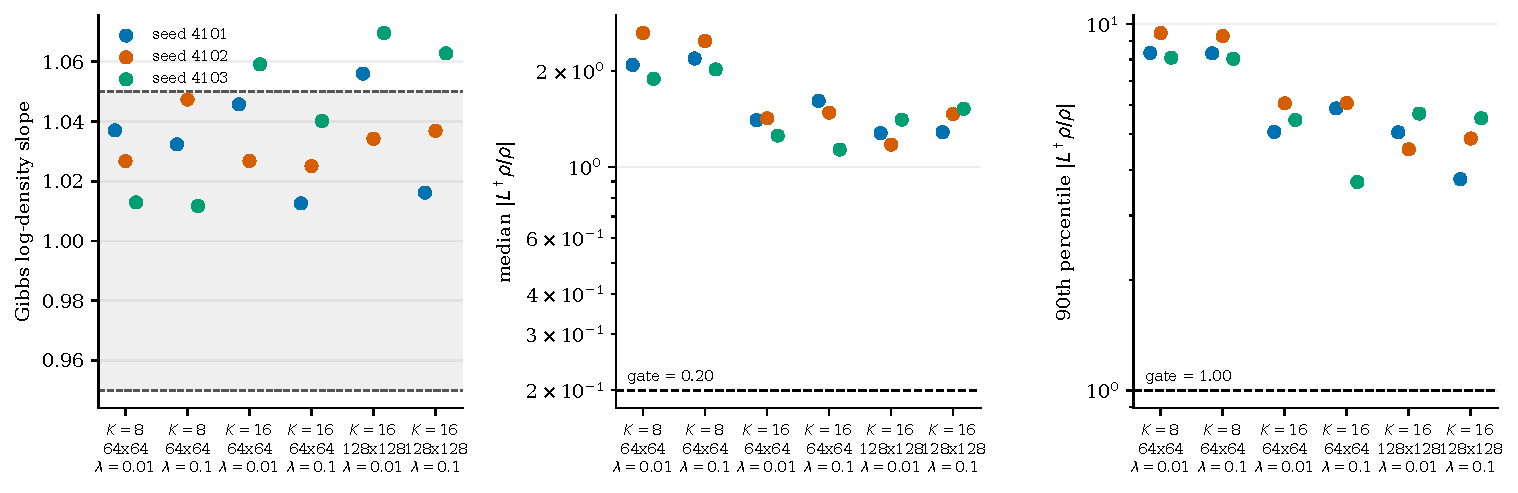
\includegraphics[width=\textwidth]{../figures/equilibrium_density_candidate_gates.pdf}
\caption{Complete equilibrium validation matrix.  The slope alone can look
reasonable while the pointwise stationary-equation residual fails by a large
factor.  Each point is one independently trained seed.}
\end{figure}

\begin{table}[p]
\centering
\caption{Equilibrium validation summaries; each row contains three seeds.}
\resizebox{\textwidth}{!}{%
\begin{tabular}{@{}rrrcccccc@{}}
\toprule
$K$ & widths & $\lambda_{\rm FP}$ & median NLL & Gibbs slope & centered RMSE & median residual & p90 residual & admissible \\
\midrule
8  & 64x64   & 0.01 & 7.9010 & [1.0129,1.0370] & [0.4558,0.5471] & [1.886,2.624] & [8.096,9.456] & no \\
8  & 64x64   & 0.10 & 7.9487 & [1.0117,1.0474] & [0.5454,0.5954] & [2.018,2.478] & [8.044,9.277] & no \\
16 & 64x64   & 0.01 & 7.8255 & [1.0268,1.0592] & [0.3034,0.3520] & [1.253,1.419] & [5.075,6.075] & no \\
16 & 64x64   & 0.10 & 7.9112 & [1.0126,1.0401] & [0.4646,0.5319] & [1.133,1.610] & [3.705,6.085] & no \\
16 & 128x128 & 0.01 & 7.8291 & [1.0342,1.0696] & [0.3020,0.3533] & [1.174,1.406] & [4.552,5.698] & no \\
16 & 128x128 & 0.10 & 7.9494 & [1.0162,1.0628] & [0.4511,0.5860] & [1.285,1.520] & [3.772,5.529] & no \\
\bottomrule
\end{tabular}}
\end{table}

\paragraph{Verdict.} \fail.  The best median residual is 1.133, 5.7 times the
declared 0.20 gate; the best p90 residual is 3.705, 3.7 times its gate.  The
selector therefore returned \code{NO\_ADMISSIBLE\_CANDIDATE}.  Following the
registered stop rule, we did not inspect the equilibrium density blind split
and did not train a driven density.  The present model family does not support
a claim that the five-dimensional stationary Fokker--Planck equation has been
numerically solved.

\section{Implication for the stabilization subsection}

The density failure does not invalidate the controlled stationary
trajectories: their operator, ESS, and regular weak-identity checks pass.  It
does prevent us from assigning quantitative probability to high- and
low-energy regions using this neural density.  Thus a density-based
stabilization mechanism is \na.  It should be revisited only with either a new
model class that independently passes the same equilibrium calibration, or
with directly estimable conditional balance observables and separately frozen
controls.

\section{Held-out generator modes}

The mode branch was run independently.  EDMD operators were fitted on 32
streams, selected on 16 validation streams, frozen, and evaluated once on 16
test streams.  The slow real mode used $\tau=0.5$.  The targeted exchange-odd
complex mode used $\tau=0.05$, safely below its principal-log Nyquist limit.

\begin{figure}[p]
\centering
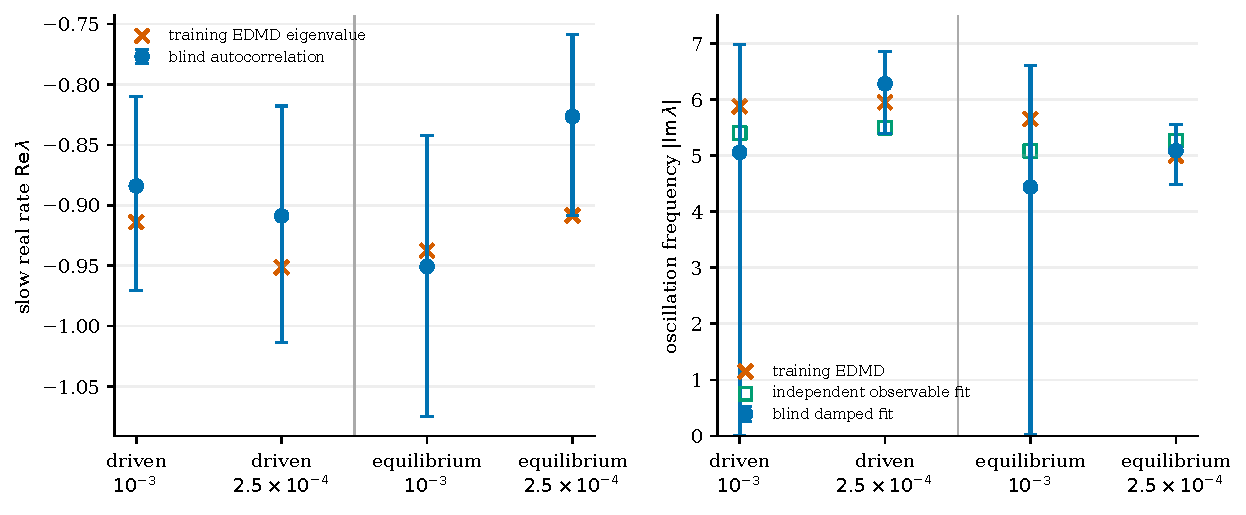
\includegraphics[width=\textwidth]{../figures/heldout_relaxation_modes.pdf}
\caption{Training EDMD eigenvalues compared with independent blind-trajectory
rate measurements.  The coarse-step oscillatory intervals are broad; the fine
step provides the useful precision.}
\end{figure}

\begin{table}[p]
\centering
\caption{Held-out mode measurements.  Residuals are test/validation.}
\resizebox{\textwidth}{!}{%
\begin{tabular}{@{}llcccc@{}}
\toprule
Bath & $dt$ & blind real rate [95\% CI] & blind frequency [95\% CI] & residuals & interpretation \\
\midrule
driven & $10^{-3}$ & $-0.884$ [$-0.971,-0.810$] & 5.059 [0.0003,6.983] & 0.807/0.850 & coarse frequency broad \\
driven & $2.5\times10^{-4}$ & $-0.909$ [$-1.014,-0.818$] & 6.281 [5.388,6.862] & 0.668/0.733 & resolved \\
equilibrium & $10^{-3}$ & $-0.951$ [$-1.075,-0.842$] & 4.438 [0.024,6.604] & 0.751/0.794 & coarse frequency broad \\
equilibrium & $2.5\times10^{-4}$ & $-0.826$ [$-0.908,-0.759$] & 5.088 [4.487,5.558] & 0.695/0.713 & resolved \\
\bottomrule
\end{tabular}}
\end{table}

The real-mode blind intervals overlap between timesteps for each bath
condition.  The fine-step frequencies agree with independent fits (5.500
driven and 5.264 equilibrium), and the damped model is strongly preferred by
AIC.  These are held-out validations of modes visible to the frozen EDMD
dictionary.

\begin{figure}[p]
\centering
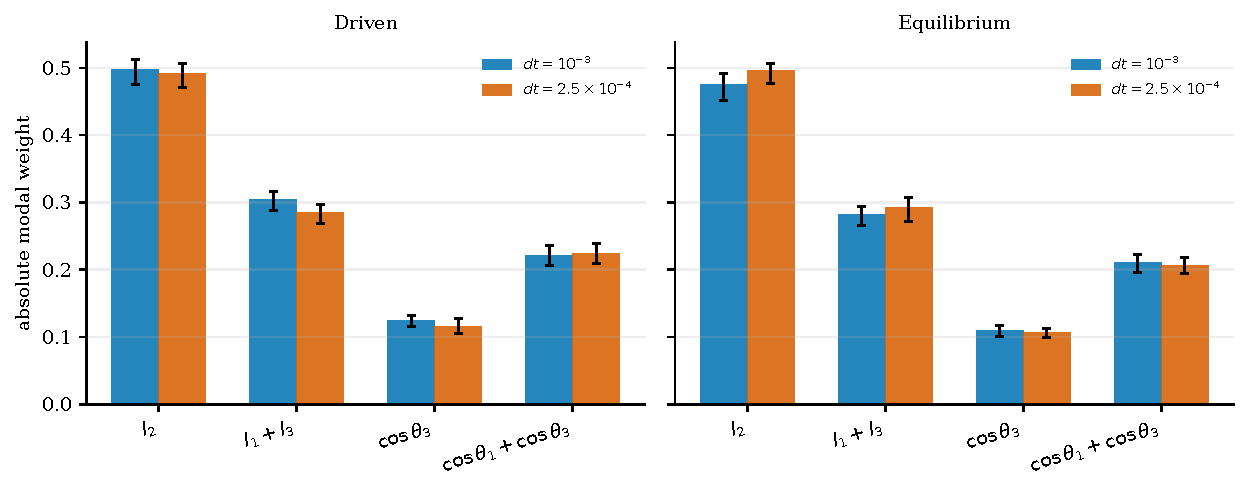
\includegraphics[width=\textwidth]{../figures/blind_slow_mode_weights.pdf}
\caption{Absolute observable weights in the frozen slow real mode.  Error bars
are 95\% whole-trajectory bootstrap intervals.}
\end{figure}

The slow-mode weight ordering is stable: $I_2$ (0.47--0.50), $I_1+I_3$
(0.28--0.30), the cosine sum (0.20--0.22), and $\cos\theta_3$
(0.106--0.124).  This explains the different visibility of the slow mode in
raw observables.  Nevertheless, the preregistered common-autocorrelation-
plateau gate remains false.  The validated real mode must therefore be called
an \emph{EDMD-visible slow mode}, not the unique spectral gap of the full
generator.

\section{Audit trail and claim boundary}

All analysis-time repairs are documented before the affected rerun:
float64 direct-state output, serialization-only model saving, selector
filtering of preserved failed-save directories, generator-domain correction of
the weak family, and the deterministic modal-weight read.  None changes a
scientific threshold or selects a result by closeness to a target.

\begin{center}
\fbox{\begin{minipage}{0.93\textwidth}
\textbf{Permitted claim.} The controlled three-mode trajectories support a
held-out EDMD-visible slow real mode and a faster damped oscillation.  The
tested normalized neural density family fails the equilibrium Gibbs/
Fokker--Planck known-answer calibration; therefore the full NESS density,
density-derived stabilization mechanism, and unique spectral gap remain
unresolved.
\end{minipage}}
\end{center}

\end{document}
